% Options for packages loaded elsewhere
\PassOptionsToPackage{unicode}{hyperref}
\PassOptionsToPackage{hyphens}{url}
%
\documentclass[
]{article}
\title{Modeling the effect of temperature on fish growth in the
California Current}
\author{Paul Spencer\footnote{\href{mailto:paul.spencer@noaa.gov}{\nolinkurl{paul.spencer@noaa.gov}},
  Alaska Fisheries Science Center, National Marine Fisheries Service,
  XXXX Sandpoint Way, Seattle, WA XXXXX, USA} \and Tara
Marshall\footnote{UK} \and Alan Boudron\footnote{UK} \and Timothy J.
Miller\footnote{Northeast Fisheries Science Center, National Marine
  Fisheries Service, 166 Water Street, Woods Hole, MA 02543, USA} \and Christine
Stawitz\footnote{Office of Science and Technology, National Marine
  Fisheries Service, Sand Point Way, Seattle, USA} \and Melissa
Haltuch\footnote{Northwest Fisheries Science Center, National Marine
  Fisheries Service, Montlake Blvd, Seattle, WA XXXXX, USA}}
\date{}

\usepackage{amsmath,amssymb}
\usepackage{lmodern}
\usepackage{iftex}
\ifPDFTeX
  \usepackage[T1]{fontenc}
  \usepackage[utf8]{inputenc}
  \usepackage{textcomp} % provide euro and other symbols
\else % if luatex or xetex
  \usepackage{unicode-math}
  \defaultfontfeatures{Scale=MatchLowercase}
  \defaultfontfeatures[\rmfamily]{Ligatures=TeX,Scale=1}
\fi
% Use upquote if available, for straight quotes in verbatim environments
\IfFileExists{upquote.sty}{\usepackage{upquote}}{}
\IfFileExists{microtype.sty}{% use microtype if available
  \usepackage[]{microtype}
  \UseMicrotypeSet[protrusion]{basicmath} % disable protrusion for tt fonts
}{}
\makeatletter
\@ifundefined{KOMAClassName}{% if non-KOMA class
  \IfFileExists{parskip.sty}{%
    \usepackage{parskip}
  }{% else
    \setlength{\parindent}{0pt}
    \setlength{\parskip}{6pt plus 2pt minus 1pt}}
}{% if KOMA class
  \KOMAoptions{parskip=half}}
\makeatother
\usepackage{xcolor}
\IfFileExists{xurl.sty}{\usepackage{xurl}}{} % add URL line breaks if available
\IfFileExists{bookmark.sty}{\usepackage{bookmark}}{\usepackage{hyperref}}
\hypersetup{
  pdftitle={Modeling the effect of temperature on fish growth in the California Current},
  pdfauthor={Paul Spencer; Tara Marshall; Alan Boudron; Timothy J. Miller; Christine Stawitz; Melissa Haltuch},
  hidelinks,
  pdfcreator={LaTeX via pandoc}}
\urlstyle{same} % disable monospaced font for URLs
\usepackage[margin=1in]{geometry}
\usepackage{graphicx}
\makeatletter
\def\maxwidth{\ifdim\Gin@nat@width>\linewidth\linewidth\else\Gin@nat@width\fi}
\def\maxheight{\ifdim\Gin@nat@height>\textheight\textheight\else\Gin@nat@height\fi}
\makeatother
% Scale images if necessary, so that they will not overflow the page
% margins by default, and it is still possible to overwrite the defaults
% using explicit options in \includegraphics[width, height, ...]{}
\setkeys{Gin}{width=\maxwidth,height=\maxheight,keepaspectratio}
% Set default figure placement to htbp
\makeatletter
\def\fps@figure{htbp}
\makeatother
\setlength{\emergencystretch}{3em} % prevent overfull lines
\providecommand{\tightlist}{%
  \setlength{\itemsep}{0pt}\setlength{\parskip}{0pt}}
\setcounter{secnumdepth}{5}
\newlength{\cslhangindent}
\setlength{\cslhangindent}{1.5em}
\newlength{\csllabelwidth}
\setlength{\csllabelwidth}{3em}
\newlength{\cslentryspacingunit} % times entry-spacing
\setlength{\cslentryspacingunit}{\parskip}
\newenvironment{CSLReferences}[2] % #1 hanging-ident, #2 entry spacing
 {% don't indent paragraphs
  \setlength{\parindent}{0pt}
  % turn on hanging indent if param 1 is 1
  \ifodd #1
  \let\oldpar\par
  \def\par{\hangindent=\cslhangindent\oldpar}
  \fi
  % set entry spacing
  \setlength{\parskip}{#2\cslentryspacingunit}
 }%
 {}
\usepackage{calc}
\newcommand{\CSLBlock}[1]{#1\hfill\break}
\newcommand{\CSLLeftMargin}[1]{\parbox[t]{\csllabelwidth}{#1}}
\newcommand{\CSLRightInline}[1]{\parbox[t]{\linewidth - \csllabelwidth}{#1}\break}
\newcommand{\CSLIndent}[1]{\hspace{\cslhangindent}#1}
\usepackage{url}
\usepackage{setspace}
%\singlespacing
%\onehalfspacing
\doublespacing
\usepackage{lineno}
\linenumbers
\usepackage[belowskip=0pt,aboveskip=0pt]{caption}
\usepackage{relsize}
\newcommand{\afrb}{Alaska Fishery Research Bulletin\xspace}
\newcommand{\ajms}{African Journal of Marine Science\xspace}
\newcommand{\amb}{Advances in Marine Biology\xspace}
\newcommand{\bms}{Bulletin of Marine Science\xspace}
\newcommand{\bjssf}{Bulletin of the Japanese Society of Scientific Fisheries\xspace}
\newcommand{\cb}{Conservation Biology\xspace}
\newcommand{\cjfas}{Canadian Journal of Fisheries and Aquatic Sciences\xspace}
\newcommand{\ea}{Ecological Applications\xspace}
\newcommand{\eer}{Evolutionary Ecology Research\xspace}
\newcommand{\elet}{Ecology Letters\xspace}
\newcommand{\emod}{Ecological Modelling\xspace}
\newcommand{\ebf}{Environmental Biology of Fishes\xspace}
\newcommand{\ff}{Fish and Fisheries\xspace}
\newcommand{\fo}{Fisheries Oceanography\xspace}
\newcommand{\fr}{Fisheries Research\xspace}
\newcommand{\fb}{Fishery Bulletin\xspace}
\newcommand{\ijms}{ICES Journal of Marine Science\xspace}
\newcommand{\iccat}{Collective Volume of Scientific Papers ICCAT\xspace}
\newcommand{\jae}{Journal of Animal Ecology\xspace}
\newcommand{\jai}{Journal of Applied Ichthyology\xspace}
\newcommand{\jdc}{Journal Du Conseil International Pour L'exploration De La Mer\xspace}
\newcommand{\jdcp}{Journal Du Conseil Permanent International Pour L'exploration De La Mer\xspace}
\newcommand{\jembe}{Journal of Experimental Marine Biology and Ecology\xspace}
\newcommand{\jfb}{Journal of Fish Biology\xspace}
\newcommand{\jsr}{Journal of Sea Research\xspace}
\newcommand{\jtb}{Journal of Theoretical Biology\xspace}
\newcommand{\jfrbc}{Journal of the Fisheries Research Board of Canada\xspace}
\newcommand{\jnwafs}{Journal of Northwest Atlantic Fisheries Science\xspace}
\newcommand{\mcf}{Marine and Coastal Fisheries: Dynamics, Management, and Ecosystem Science\xspace}
\newcommand{\mb}{Marine Biology\xspace}
\newcommand{\meps}{Marine Ecology Progress Series\xspace}
\newcommand{\mfr}{Marine Fisheries Review\xspace}
\newcommand{\mpb}{Marine Pollution Bulletin\xspace}
\newcommand{\najfm}{North American Journal of Fisheries Management\xspace}
\newcommand{\nzjmfr}{New Zealand Journal of Marine and Freshwater Research\xspace}
\newcommand{\pnas}{Proceedings of the National Academy of Sciences USA\xspace}
\newcommand{\rpvrciemm}{Rapports et Proc\`es-Verbaux des R\'eunions. Conseil Internationale pour l'Exploration de la Mer\xspace}
\newcommand{\rpvrcpiemm}{Rapports et Proc\`es-Verbaux des R\'eunions. Conseil Permanent Internationale pour l'Exploration de la Mer\xspace}
\newcommand{\rfbf}{Reviews in Fish Biology and Fisheries\xspace}
\newcommand{\sajms}{South African Journal of Marine Science\xspace}
\newcommand{\tafs}{Transactions of the American Fisheries Society\xspace}

\newcommand{\anzjs}{Australian \& New Zealand Journal of Statistics\xspace}
\newcommand{\as}{Applied Statistics\xspace}
\newcommand{\csda}{Computational Statistics \& Data Analysis\xspace}
\newcommand{\ees}{Environmental and Ecological Statistics\xspace}
\newcommand{\jas}{Journal of Applied Statistics\xspace}
\newcommand{\jabes}{Journal of Agricultural, Biological, and Environmental Statistics\xspace}
\newcommand{\jasa}{Journal of the American Statistical Association\xspace}
\newcommand{\jrssb}{Journal of the Royal Statistical Society. Series B\xspace}
\newcommand{\sm}{Statistics in Medicine}

\usepackage{xspace}
\usepackage{bm}
\usepackage{caption,graphics}
\usepackage{graphicx}
\usepackage{makecell}
\renewcommand\figurename{Fig.}
\captionsetup{labelsep=period, singlelinecheck=false}
\usepackage{footmisc}
\newcommand{\changesize}[1]{\fontsize{#1pt}{#1pt}\selectfont}
\renewcommand{\arraystretch}{1.5}
\renewcommand\theadfont{}
\usepackage{booktabs}
\usepackage{longtable}
\usepackage{array}
\usepackage{multirow}
\usepackage{wrapfig}
\usepackage{float}
\usepackage{colortbl}
\usepackage{pdflscape}
\usepackage{tabu}
\usepackage{threeparttable}
\usepackage{threeparttablex}
\usepackage[normalem]{ulem}
\usepackage{makecell}
\usepackage{xcolor}
\ifLuaTeX
  \usepackage{selnolig}  % disable illegal ligatures
\fi

\begin{document}
\maketitle

\pagebreak

\hypertarget{abstract}{%
\subsection*{Abstract}\label{abstract}}
\addcontentsline{toc}{subsection}{Abstract}

\hypertarget{keywords}{%
\subsubsection*{Keywords}\label{keywords}}
\addcontentsline{toc}{subsubsection}{Keywords}

growth; climate; stock assessment; reference points

\pagebreak

\hypertarget{introduction}{%
\section{Introduction}\label{introduction}}

The somatic growth of individual fish, from larval to adult stages,
underpins the size structuring of aquatic ecosystems and is also subject
to environmental influences (Black 2009). Growth is an inherently
non-linear process resulting from dynamic fluxes between anabolism and
catabolism (Quinn and Deriso 1999). Consequently, abrupt changes in
growth rates can occur throughout the lifespan of an individual fish,
most notably during the transition between the rapid growth of juvenile
stages and the slower growth during adult stages {[}Lester et al.
(2004);quinceetal08{]}. Dynamic changes in size-at-age can have direct
impacts on rates of harvest and fishery management reference points
because fisheries management is often based on limiting mortality (i.e.,
based on abundance) via biomass-based harvest quotas and the assumption
of an average growth relationship through time (Miller et al. 2018).
However, if growth fluctuates well above or below the long term average
growth relationship then realized biomass-based harvest quotas may be
lower or higher than quotas set as a function of an average growth
relationship. The dominant patterns in and magnitudes of somatic growth
variation over long time scales have not been quantified for many
commercially important fish stocks (Stawitz et al. 2015). Therefore,
quantifying the basic characteristics and dominant scales of variation
in growth is the necessary first step towards predicting growth
responses to biotic and abiotic factors (Stawitz et al. 2015).

Individual growth rates vary on a range of temporal and biological
scales, including across species and populations of the same species
(Brander 1995, Brunel and Dickey-Collas 2010). Within a given system,
variation in size-at-age may occur between cohorts of a single
population (Baudron et al.~2011, Baudron et al.~2014), between years, or
between juveniles of cohorts (Stawitz et al. 2015). Understanding the
variation in size-at-age can help refine mechanistic hypotheses.
Density-independent annual changes in growth may occur from processes
such as upwelling, affecting all ages within a year. Alternatively,
density-dependent processes such as intracohort competition may affect
strong cohorts; in this case, environmental processes that lead to
strong recruitment may result in reduced growth rates (Whitten et
al.~2013). A third mechanism is that variability in growth is related to
only the size-at-age of juvenile fish, with growth rates of older ages
unaffected by the environment, which is consistent with juvenile
intracohort competition being the dominant process. Stawitz et
al.~(2015) examined these hypotheses for North Pacific groundfish, and
found that about 40\% of the stocks studied showed density-independent
annual growth variation between years.

Because temperature is an important determinant of growth for
ectothermic species, the temperature size rule (TSR) provides the basis
for an important hypothesis relevant to climate change. The temperature
size rule (TSR) proposes that juvenile growth rates are higher in warmer
waters due to higher metabolic rates with rapid early growth leading to
a lower maximum (adult) size-at-age (Angilletta et al.~2004, Daufresne
et al.~2009, Forster and Hirst 2012, Forster et al.~2011). In the
context of warming regional seas, the TSR has the potential for imposing
a low-frequency signal into variability in individual growth rates of
fish. For example, warming temperatures in the North Sea imposed a
synchronous cross-species trend in growth rates of 6 of 8 commercial
fish stocks consistent with the TSR (Baudron et al.~2014). A combination
of temperature-related reductions in body size and distributional shifts
has been estimated to reduce fisheries yields by as much as 25\% (Cheung
et al.~2013).

The von Bertalanffy growth function (VBGF; von Bertalanffy 1938),
developed from physiological concepts such as catabolism and anabolism
(Essington et al.~2001), can be used to test how temperature may affect
size-at-age and potentially particular aspects (e.g., parameters) of the
growth process. Simple correlations between temperature and the VBGF
have been undertaken (Brunel and Dickey-Collas 2010), an approach that
would require temperature impacts to be strong relative to other sources
of variation. Adaptations of the VBGF have been developed to incorporate
the effect of temperature and other environmental factors directly into
the VBGF parameters \(L_\infty\) (asymptotic size) and K (rate at which
\(L_\infty\) is approached) (Fontoura and Agostinho 1996, Shin and
Rochet 1998). Kimura (2008) developed an extended form of the VBGF which
could include any explanatory variable as a covariate, which (Baudron et
al.~2011) used to determine that temperature was a statistically
significant covariate in the cohort-specific VBGF fit for North Sea
haddock stock. Although the VBGF has the advantage of allowing
consideration of how environmental variability affects specific aspects
of growth, estimation of changes in both the k and \(L_\infty\)
parameters is difficult because they are highly correlated (Schnute and
Fournier 1980).

Rapid and variable local responses of fish size to warming can also make
temperature responses difficult to diagnose and predict at the ecosystem
scale (Audzijonyte et al.~2020). Testing for a coherent (sensu
consistent with established physiology of ectotherms and widely observed
across different species) biological response to temperature at the
ecosystem scale requires using a statistical model suited to isolating
the impacts of a single, external factor (i.e., temperature) on fish
growth rates in addition to other possible sources of variation (e.g.,
density, prey abundance, fisheries-induced changes in life history).
Coherent and synchronous annual growth trends across species that are
consistent with physiological principles (e.g., TSR) would imply there
is a component of growth variation that is a shared response to
ecosystem-scale warming (Baudron et al.~2014, Stawitz et al.~2015).
Isolating such a response at the stock- or ecosystem-level would provide
the necessary empirical support for models developed to forecast future
fish yields (e.g., Cheung et al.~2013). Because ecosystem observations
do not come from controlled experiments in which variables of interest
can be isolated, more complex statistical methods will be necessary to
evaluate any potential coherent, cross-species signal in the effect of
temperature on growth. An additional consideration is whether to model
observation errors, which is particularly relevant because the data
available are typically observations of size-at-age from individual fish
(i.e., multiple observations of size-at-age from a single fish that
would more clearly show individual growth are typically not available).
Temporal trends in size-at-age data could reflect trends in gear
selectivity, sampling locations, ageing bias and precision, and other
factors. A closely related concept is whether to employ Bayesian or
random-effects methods that would model observations and/or estimated
parameters as random variables. For example, changes in sampling
location or the effect of environmental covariates on size can be
modeled as random variables to account for unobserved heterogeneity not
explained by the structural model.

A variety of advanced statistical techniques have been applied recently
to evaluate variation in fish size-at-age. (Baudron et al.~2014) used
Dynamic Factor Analysis (DFA; Zuur et al 2003) to estimate common
``latent'' trends in the cohort-specific \(L_\infty\) time series for
eight North Sea stocks with long time series of size-at-age. DFA is a
multivariate extension of structural time series, with the time series
for a particular stock being a function of underlying latent trends and
stock-specific observation error. An alternative framework applied by
(Stawitz et al.~2015) are autoregressive state-space models consisting
of process and observation models that fit to observed time series of
standardized length-at-age data without a mechanistic growth model.
Miller et al.~(2018) also used a state-space model, but the process
model is based on a generalized VBGF that allowed process errors in the
k parameter. Finally, spatio-temporal models such as VAST (Vector
Autoregressive Spatio-Temporal model; www.github.com/james-thorson/VAST)
are mixed-effect models in which model spatial variation as random
effects given a pattern of spatial correlation, and a number of
covariates can be modeled as fixed effects. Although VAST models are
often applied to data on fish density from resource surveys (Thorson
2019), they can be potentially useful for cases where fish size-at-age
may vary over space in patterns not related to the modeled fixed
effects.

An alternative framework that has been applied to modelling individual
growth is autoregressive state-space models that compare the relative
importance of different scales of variation (e.g., annual, cohort) and
extract underlying growth trends across species (Stawitz et al. 2015).
State-space models simultaneously estimate model parameters using two
equations: the autoregressive process representing abiotic and biotic
covariates and the unobserved processes including space and time
covariates.

The inferences that can be made regarding how temperature affects fish
growth are influenced by the choice of model structure. In particular,
evaluation of a series of models may help illuminate modeling approaches
that have utility when any coherent response of fish growth to
temperature may be subtle relative to asynchronous or stock-specific
factors (e.g., food availability, density). Although the models
mentioned above all have a common property of recognizing variation
other than the ``process'' variation of interest, they apportion
variance very differently because of differences in model structure.
Multi-model inference is the process whereby the response variable is
estimated using several candidate models rather than a single `best'
model (Burnham and Anderson 2002) and has been previously applied to
growth modelling (Katsanevakis and Maravelias 2008). In our study the
intent was not necessarily to predict the response variable with the
greatest accuracy but to identify the modelling framework(s) best suited
to assessing whether there was a synchronous impact of temperature once
other sources of variation have been accounted for (state-space models)
or once asynchronous sources of variation had been excluded (DFA).
Comparative analysis of models can also help to identify biases in model
performance (e.g.~whether a model systematically underestimates random
noise in the data) or shortcomings in model fitting (e.g., estimation of
process or observation error). For example, Brodie et al.~(2020)
compared several types of species distribution models and identified
which models were appropriate for specific purposes. Ultimately model
purpose must be given due consideration when deciding on the most
appropriate modelling framework (Brodie et al.~2020, Guillera-Arroita et
al.~2015).

The aim of this study is to undertake a comparative analysis of four
models using empirical data for temperature and size-at-age for seven
fish stocks in the California Current large marine ecosystem. A common
metric for the models is to evaluate the degree to which size-at-age is
related to temperature. Estimates of uncertainties, parameter
correlations, and any potential aliasing (i.e., erroneously attributing
variation size-at-age to non-causal mechanisms or covariates). We
consider the relative strength and weakness of the models in describing
how temperature may affect size-at-age, and how the combination of
models can be used for multi-model inference.

\hypertarget{methods}{%
\section{Methods}\label{methods}}

\hypertarget{study-area-species-chosen-trawl-survey-description-melissa-feb-29}{%
\subsection{Study area, species chosen, trawl survey description
(Melissa, Feb
29)}\label{study-area-species-chosen-trawl-survey-description-melissa-feb-29}}

Four trawl surveys conducted by the National Marine Fisheries Center's
Alaska Fisheries Science Center (AFSC) and Northwest Fisheries Science
Center (NWFSC) provided data for this study. The Triennial Shelf Survey,
conducted by the AFSC in 1980, 1983, 1986, 1989, 1992, 1995, 1998, and
2001 and by the NWFSC in 2004, provides the earliest time series of
fishery independent temperature and biological data in the U.S. portion
of the California Current continental shelf (Weinberg et al. 2002).
Triennial survey sampling occurred along transects perpendicular to the
coast over depths from 55 m to 366 m (500 m after 1992) and from the
Canadian border to Monterey Bay, California (36°48' N) until 1986, then
to Point Conception, California (34°30' N) from 1989 forward.

The transect-based AFSC Slope Survey was conducted in 1997, 1999, 2000,
and 2001, over depths from 184 m to 1,280 m in waters north of Point
Conception, California (34°30' N) to the US -- Canada border (Lauth
1999, 2000, 2001). Sampling in earlier years was spatially limited,
covering small and inconsistent portions of the coast; however, this
survey had a high degree of biological sampling.

The transect-based NWFSC Slope survey, conducted in 1998, 1999, 2000,
2001, and 2002, covered depths ranging from 184 m to 1,280 m using
chartered commercial fishing vessels \textless93 feet (Keller et al.
2017). Prior to 2000 the NWFSC Slope survey sampled from the Morro Bay,
California (lat 35°00'N), to the U.S.--Canada border, the survey area
was expanded south to Point Conception, California (34°30' N) in 2001,
then to the U.S. Mexico border in 2002. This survey consists of fewer
tows compared to other survey data sets, with a lower fraction of tows
sampled for ages.

The NWFSC West Coast Groundfish Bottom Trawl Survey (WCGBTS), operating
annually from 2003 through 2019, implements a stratified random-grid
survey design that spans both continental shelf and slope habitats,
depths from 55m to 1,280 m, and covers U.S. waters between the Canada
and Mexico borders (Bradburn et al. 2011; Keller et al. 2017). Strata
include three depth strata (55 m to 183 m, 184 m to 549 m, and 550 m
to1280 m) and two spatial strata (north and south of Point Conception,
California (34°30' N)) for all years except 2003. In 2003 five spatial
strata delineated by the boundaries of the International North Pacific
Fisheries Commission (INPFC) statistical areas were used. These INPFC
statistical areas are, from north to south, Vancouver, Columbia, Eureka,
Monterey, and Conception. Generally, four chartered industry vessels
conduct tows from late-May to early-October, in randomly selected grid
cells, during two north to south passes along the U.S. west coast.
Randomly sampled lengths and ages are collected; age structures are
sampled from a subset of the fish that have been measured for length.
Major changes in the WCGBTS, compared to prior surveys, include
implementing a stratified random survey design and consistent spatial
coverage south of Point Conception, California (34°30' N).

Regions used in this study are a combination of the 2003 WCGBTS
latitudinal and depth strata. The INPFC Vancouver, Columbia, and Eureka
latitudinal strata are combined into a single region, labeled ``ECV,''
due to ecological similarity. The combination of three INPFC latitudinal
strata and three depth strata yield nine regions defined by latitude and
depth. Mean bottom temperature used in situ data from the four surveys
for each of the nine region-year strata with at least five observations,
with data from the AFSC slope survey restricted to September -- October
to provide a similar sampling period to the remaining surveys (i.e., May
-- October).

Seven species were selected for analysis of length-at-age data, based on
a diversity of life-history traits, habitat usage, and data
availability. Length-at-age data for two deep-water species with ranges
encompassing both the continental shelf and slope (darkbloched rockfish
(\emph{Sebastes crameri}) and sablefish (\emph{Anoplopoma fimbria}))
were obtained from two surveys that collectively cover the full depth
range of these species in a given year: the Triennial Shelf Survey and
NWFSC Slope surveys for years 1998 and 2001, and the WCGBTS for the
years 2003 to 2018. Shortbelly rockfish (\emph{Sebastes jordani}) also
occur on the slope and shelf, but limited observations restricted
analysis to data from the WCGBTS. Length-at-age data for four species
that occur on the continental shelf (Pacific hake (\emph{Merluccius
productus}), Pacific sanddab (\emph{Citharichthys sordidus}), lingcod
(\emph{Ophiodon elongatus}), and petrale sole (\emph{Eopsetta jordani}))
were obtained from two surveys: the Triennial Shelf Survey and the
WCGBTS. Because marine fish stocks often change the depth and spatial
locations occupied as they age, we attempted to derive temperature time
series reflective of the habitats they occupy at a given age. We used
the species-specific set of surveys listed above to compute the mean
depth and latitude of the length-at-age samples by age (for ages 0 --
15) across years, then classified these means into the nine
latitude-depth regions. The temperature time series for a given species
and age was obtained from the corresponding latitude-depth region where
they occurred.

\hypertarget{state-space-growth-models}{%
\subsection{State-space growth models}\label{state-space-growth-models}}

We used the same general model as Miller et al. (2018) which assumes von
Bertalanffy growth and allows annual age-specific growth rates. It can
use combinations of length and weight information and simultaneously
estimates allometric length-weight relationship. We fit four alternative
models for each species (Table 1). The base model assumes the same LVB
growth rate and asymptotic size for all individuals. The second model
allows annual AR(1) deviations in the log growth rate for a given year
applied to all cohorts in that year. Allowing this AR(1) process for
annual growth rates was found by Miller et al. (2018) to be important
for evaluating effects of temperature on growth rates for Georges Bank
Atlantic cod. The third model expands the second model to include
temperature effects on the growth rate during the first year of life.
The fourth model expands the third model to allow different asymptotic
lengths for cohorts originating after 2000 when there was a dramatic
reduction in fishing pressure (Warlick et al. 2018).

For darkbotched rockfish, sablefish, and shortbelly rockfish we used
length, weight and age observations from the ``combination survey''
only, whereas for hake, sanddab, lingcod, petrale sole we used
observations from both the ``combination'' and ``trienniel'' surveys.
The total number of length and weight at age observations available for
each species ranged between 5152 for shortbelly rockfish and 17850 for
sablefish. For models and , we used the bottom temperature estimates for
the region defined by area and depth bin where the species was
predominantly found during the earliest observed ages (Table 2). We
observed age 0 fish for all species except Petrale sole (minimum age is
1), and the youngest observed ages of all species predominated in depths
less than 184 m. Young sablefish and darkblotched rockfish predominated
in the most northern region (Eureka-Columbia-Vancouver) and young
shortbelly rockfish predominated in the most southern region
(Conception). Young fish of all other species predominated in the
intermediate region (Monterey).

\hypertarget{results}{%
\section{Results}\label{results}}

\hypertarget{description-of-the-size-at-age-data-and-temperature-data-paul-feb-29}{%
\subsection{Description of the size at age data, and temperature data
(Paul, Feb
29)}\label{description-of-the-size-at-age-data-and-temperature-data-paul-feb-29}}

\hypertarget{results-from-the-4-modeling-approaches}{%
\subsection{Results from the 4 modeling
approaches}\label{results-from-the-4-modeling-approaches}}

\hypertarget{stawitz-state-space-model-christine-mar-30}{%
\subsubsection{Stawitz state-space model (Christine, Mar
30)}\label{stawitz-state-space-model-christine-mar-30}}

\hypertarget{state-space-von-bertalanffy-growth-model-tim-mar-30}{%
\subsubsection{State-space von Bertalanffy growth model (Tim, Mar
30)}\label{state-space-von-bertalanffy-growth-model-tim-mar-30}}

We found that including temperature effects on growth during the first
year of life improves model performance for all 7 species (Table 3). The
estimated temperature effect was positive for all species except
shortbelly rockfish (Table 4, Figure 1), the species with the most
southerly distribution. Allowing asymptotic size to differ for cohorts
exposed to low or high fishing pressure improved model performance for 4
of the 7 species (darkblotched rockfish, Pacific hake, sablefish, and
shortbelly rockfish). Estimates of asymptotic size for darkblotched
rockfish and Pacific hake were greater after fishing pressure was
released, but estimates were lower for sablefish and shortbelly rockfish
(Table 5).

\hypertarget{vb-dba-alan-mar-30}{%
\subsubsection{VB-DBA (Alan, Mar 30)}\label{vb-dba-alan-mar-30}}

\hypertarget{vast-model-christine-mar-30}{%
\subsubsection{VAST model (Christine, Mar
30)}\label{vast-model-christine-mar-30}}

\hypertarget{discussion}{%
\section{Discussion}\label{discussion}}

To be determined, but some organizing thoughts are:

\begin{enumerate}
\def\labelenumi{\arabic{enumi})}
\item
  Potential for attribution (and maybe misattribution) of sources of
  variability with differing modeling approaches (i.e., spatial
  vs.~non-spatial models)
\item
  Advantages/disadvantages of mechanistic models vs non-mechanistic
  models
\item
  The ability of the modeling approaches to be able to distinguish
  between the hypotheses of fish growth
\item
  The role of biology in affecting the influence of temperature on size
  at age (i.e., ontogenetic depth movement, timing of spawning
\end{enumerate}

\hypertarget{conclusion}{%
\section{Conclusion}\label{conclusion}}

\hypertarget{acknowledgements}{%
\section*{Acknowledgements}\label{acknowledgements}}
\addcontentsline{toc}{section}{Acknowledgements}

\pagebreak

\hypertarget{references}{%
\subsection*{References}\label{references}}
\addcontentsline{toc}{subsection}{References}

\hypertarget{refs}{}
\begin{CSLReferences}{1}{0}
\leavevmode\vadjust pre{\hypertarget{ref-black09}{}}%
Black, B.A. 2009. {Climate-driven synchrony across tree, bivalve, and
rockfish growth-increment chronologies of the northeast Pacific}.\meps
\textbf{378}: 37--46.
doi:\href{https://doi.org/10.3354/meps07854}{10.3354/meps07854}.

\leavevmode\vadjust pre{\hypertarget{ref-bradburnetal11}{}}%
Bradburn, M., Keller, A., and Horness, B. 2011. {The 2003 to 2008 U.S.
West Coast bottom trawl surveys of groundfish resources off Washington,
Oregon, and California: estimates of distribution, abundance, length,
and age composition}. {Tech. Rep. NMFS-NWFSC-114, U.S. Department of
Commerce, Seattle, WA}.

\leavevmode\vadjust pre{\hypertarget{ref-burnhamanderson02}{}}%
Burnham, K.P., and Anderson, D.R. 2002. Model selection and multimodel
inference: A practical information-theoretic approach. Springer-Verlag,
New York.

\leavevmode\vadjust pre{\hypertarget{ref-katsanevakis08}{}}%
Katsanevakis, S., and Maravelias, C.D. 2008. Modelling fish growth:
Multi-model inference as a better alternative to a priori using von
bertalanffy equation. Fish and Fisheries \textbf{9}(2): 178--187.
doi:\href{https://doi.org/10.1111/j.1467-2979.2008.00279.x}{10.1111/j.1467-2979.2008.00279.x}.

\leavevmode\vadjust pre{\hypertarget{ref-kelleretal17}{}}%
Keller, A.A., Wallace, J.R., and Methot, R.D. 2017. The {Northwest
Fisheries Science Center's} west coast groundfish bottom trawl survey:
History, design, and description. Seattle, WA: NOAA.

\leavevmode\vadjust pre{\hypertarget{ref-lauth99}{}}%
Lauth, R.R. 1999. The 1997 pacific west coast upper continental slope
trawl survey of groundfish resources off washington, oregon, and
california: Estimates of distribution, abundance, and length
composition. {U.S. Department of Commerce, NOAA Technical Memorandum
NMFSAFSC-98}.

\leavevmode\vadjust pre{\hypertarget{ref-lauth00}{}}%
Lauth, R.R. 2000. {The 1999 Pacific West Coast Upper Continental Slope
Trawl Survey of groundfish resources off Washington, Oregon, and
California: Estimates of distribution, abundance, and length
composition}. {U.S. Department of Commerce, NOAA Technical Memorandum
NMFSAFSC-115}.

\leavevmode\vadjust pre{\hypertarget{ref-lauth01}{}}%
Lauth, R.R. 2001. {The 2000 Pacific West Coast Upper Continental Slope
Trawl Survey of groundfish resources off Washington, Oregon, and
California: Estimates of distribution, abundance, and length
composition}. {U.S. Department of Commerce, NOAA Technical Memorandum
NMFSAFSC-120}.

\leavevmode\vadjust pre{\hypertarget{ref-lesteretal04}{}}%
Lester, N.P., Shuter, B.J., and Abrams, P.A. 2004. Interpreting the von
bertalanffy model of somatic growth in fishes: The cost of reproduction.
Proceedings of the Royal Society of London. Series B: Biological
Sciences \textbf{271}(1548): 1625--1631.
doi:\href{https://doi.org/10.1098/rspb.2004.2778}{10.1098/rspb.2004.2778}.

\leavevmode\vadjust pre{\hypertarget{ref-milleretal18}{}}%
Miller, T.J., O'Brien, L., and Fratantoni, P.S. 2018. Temporal and
environmental variation in growth and maturity and effects on management
reference points of {G}eorges {B}ank {A}tlantic cod. Canadian Journal of
Fisheries and Aquatic Sciences \textbf{75}(12): 2159--2171.
doi:\href{https://doi.org/10.1139/cjfas-2017-0124}{10.1139/cjfas-2017-0124}.

\leavevmode\vadjust pre{\hypertarget{ref-quinnderiso99}{}}%
Quinn, T.J., and Deriso, R.B. 1999. Quantitative fish dynamics. Oxford
University Press.

\leavevmode\vadjust pre{\hypertarget{ref-stawitzetal15}{}}%
Stawitz, C.C., Essington, T.E., Branch, T.A., Haltuch, M.A., Hollowed,
A.B., and Spencer, P.D. 2015. A state-space approach for detecting
growth variation and application to {N}orth {P}acific groundfish.\cjfas
\textbf{72}(9): 1316--1328.

\leavevmode\vadjust pre{\hypertarget{ref-warlicketal18}{}}%
Warlick, A., Steiner, E., and Guldin, M. 2018. {History of the West
Coast groundfish trawl fishery: Tracking socioeconomic characteristics
across different management policies in a multispecies fishery}. Marine
Policy \textbf{93}: 9--21.

\leavevmode\vadjust pre{\hypertarget{ref-weinbergetal02}{}}%
Weinberg, K.L., Wilkins, M.E., Shaw, F.R., and Zimmermann, M. 2002. The
2001 {P}acific {W}est {C}oast bottom trawl survey of groundfish
resources: Estimates of distribution, abundance, and length and age
composition. {U}.{S}. {D}epartment of {C}ommerce, {NOAA} {T}echnical
{M}emorandum {NMFS-AFSC}-128.

\end{CSLReferences}

\pagebreak

\hypertarget{appendix-a}{%
\section*{Appendix A}\label{appendix-a}}
\addcontentsline{toc}{section}{Appendix A}

\hypertarget{tables}{%
\section{Tables}\label{tables}}

\hypertarget{figures}{%
\section{Figures}\label{figures}}

\begin{figure}
\caption{Effects of bottom temperature anomaly on the von Bertelanffy growth parameter $k$ for each species.}\label{temp_effect_k}
\begin{center}
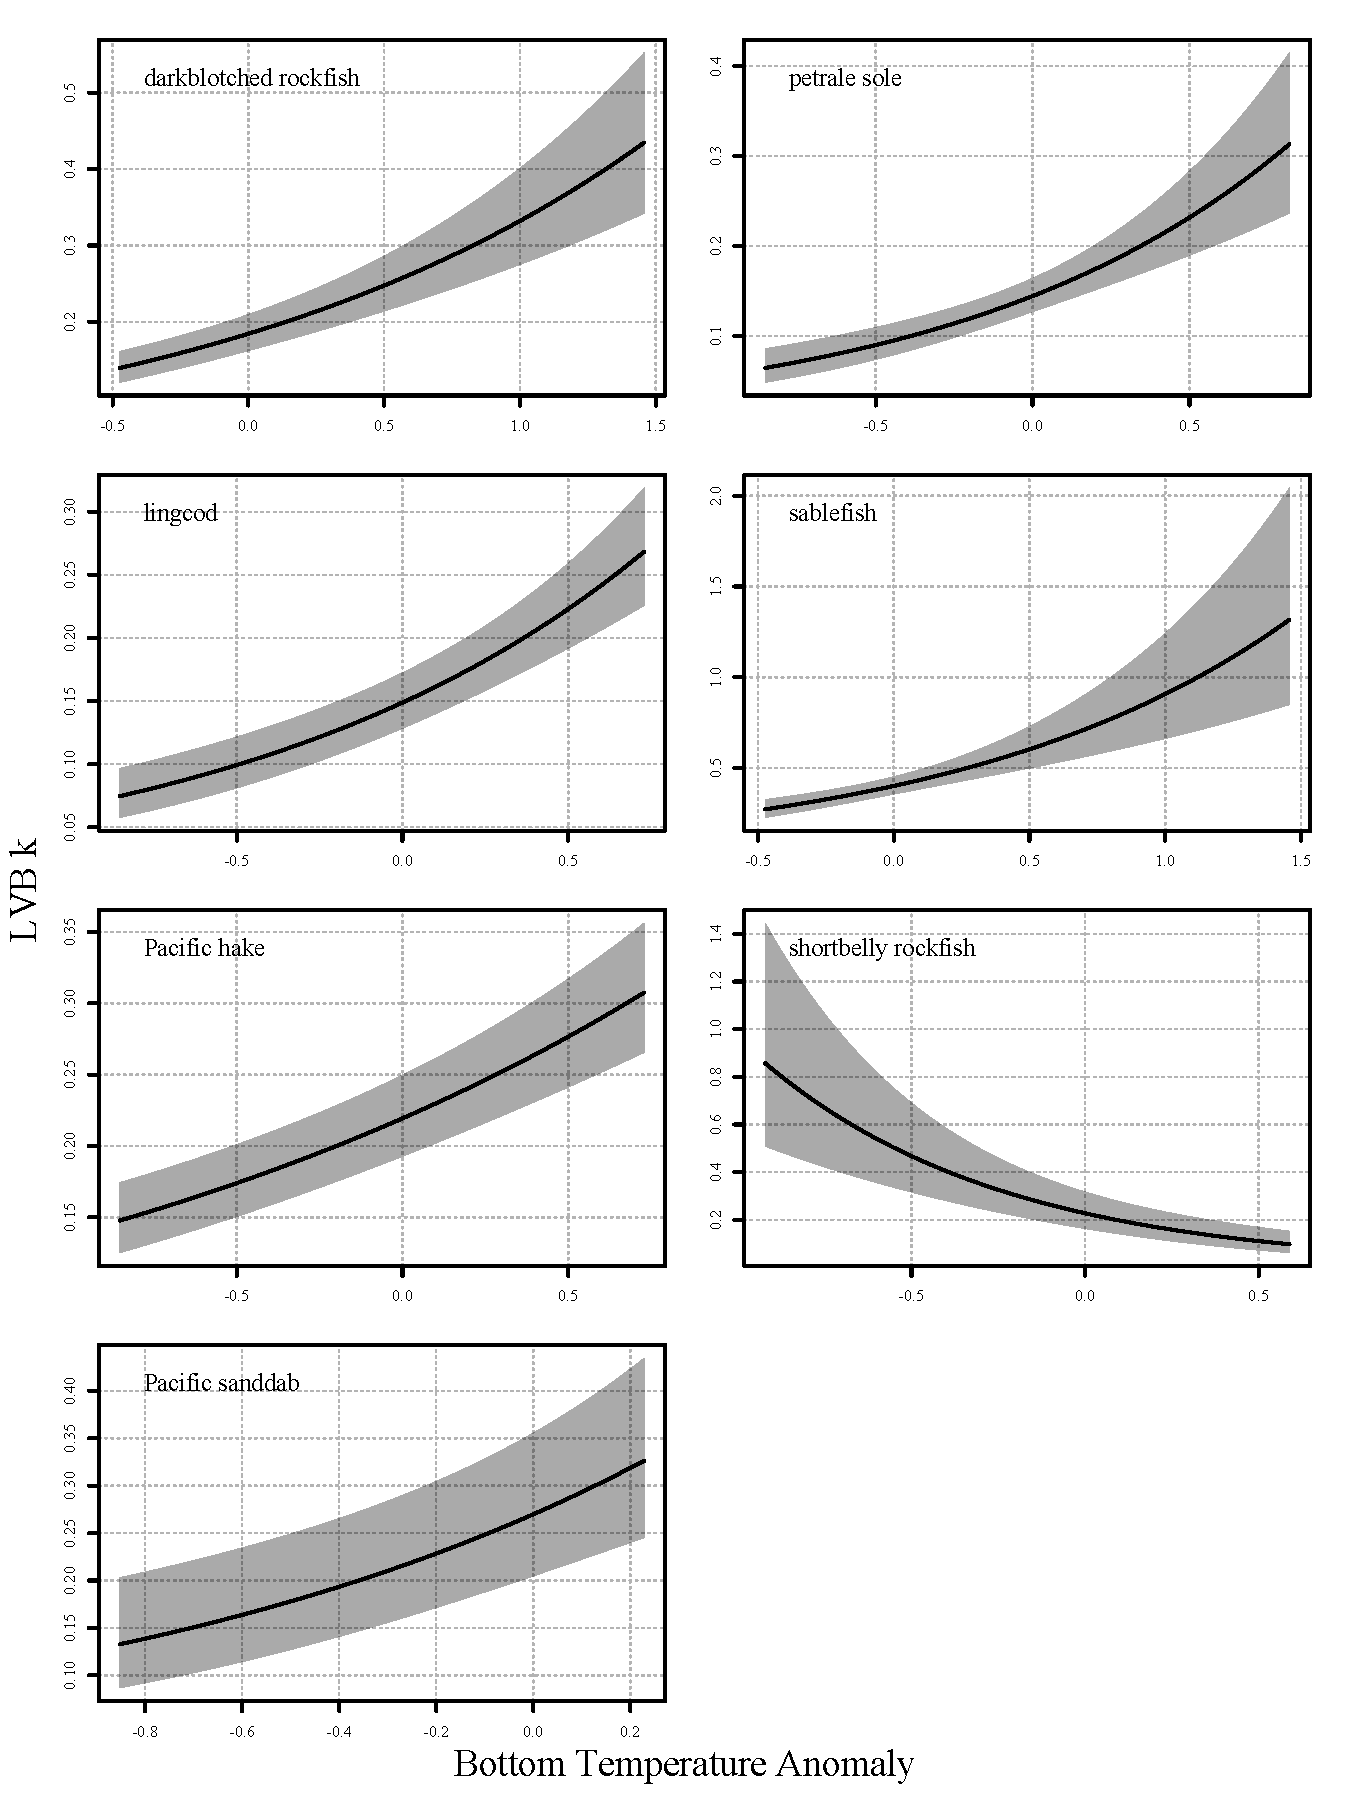
\includegraphics[height = 0.8\textheight]{../results/ss_lvb_temp/temp_effect_by_species.pdf}
\end{center}
\end{figure}

\begin{figure}
\caption{Annual spawning biomass, fully-selected fishing mortality rate, and recruitment for Petrale sole.}\label{SSB_F_R}
\begin{center}
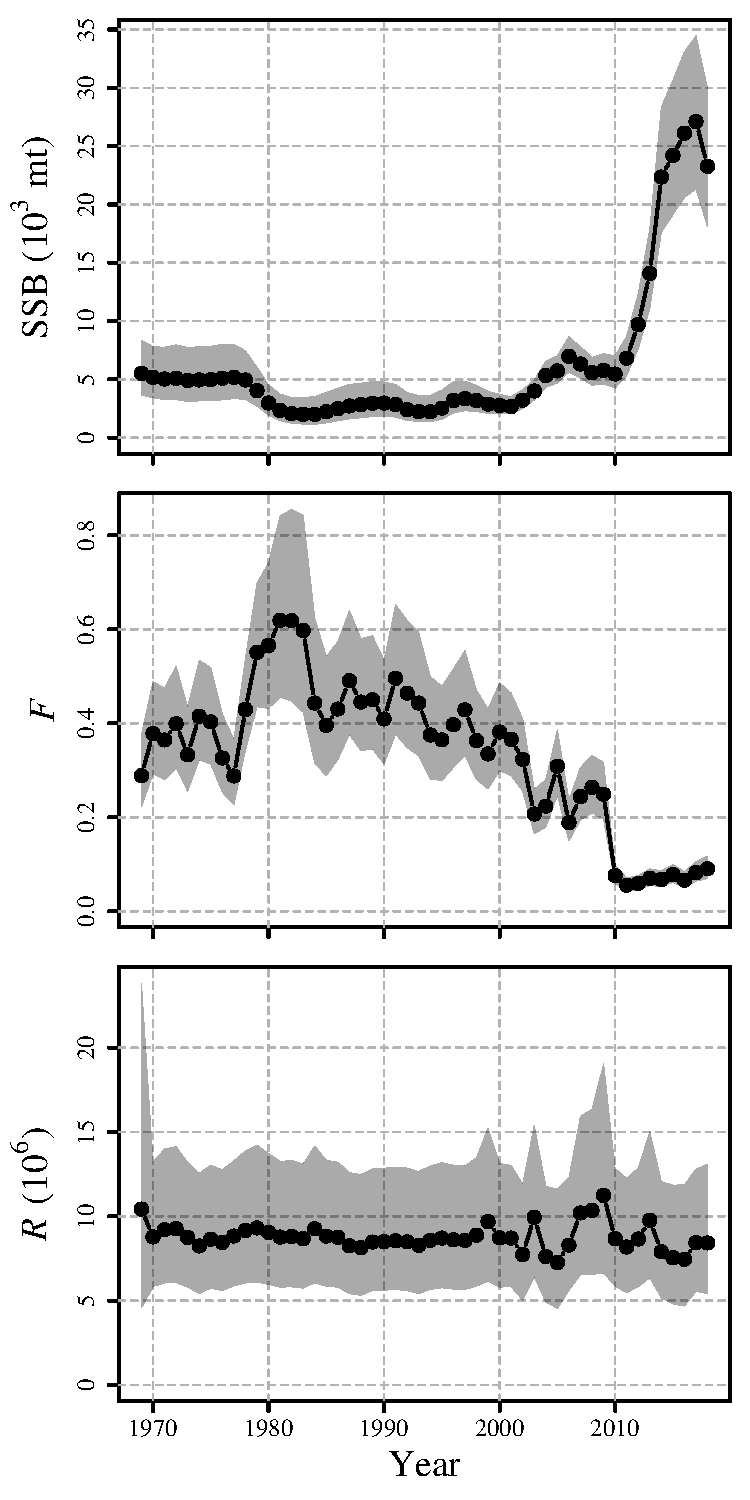
\includegraphics[height = 0.8\textheight]{../results/ssm_temp/petrale_SSB_F_R.pdf}
\end{center}
\end{figure}

\begin{figure}
\caption{Annual SSB$_{40}$ and $F_{40}$, reference points for Petrale sole.}\label{BRPs}
\begin{center}
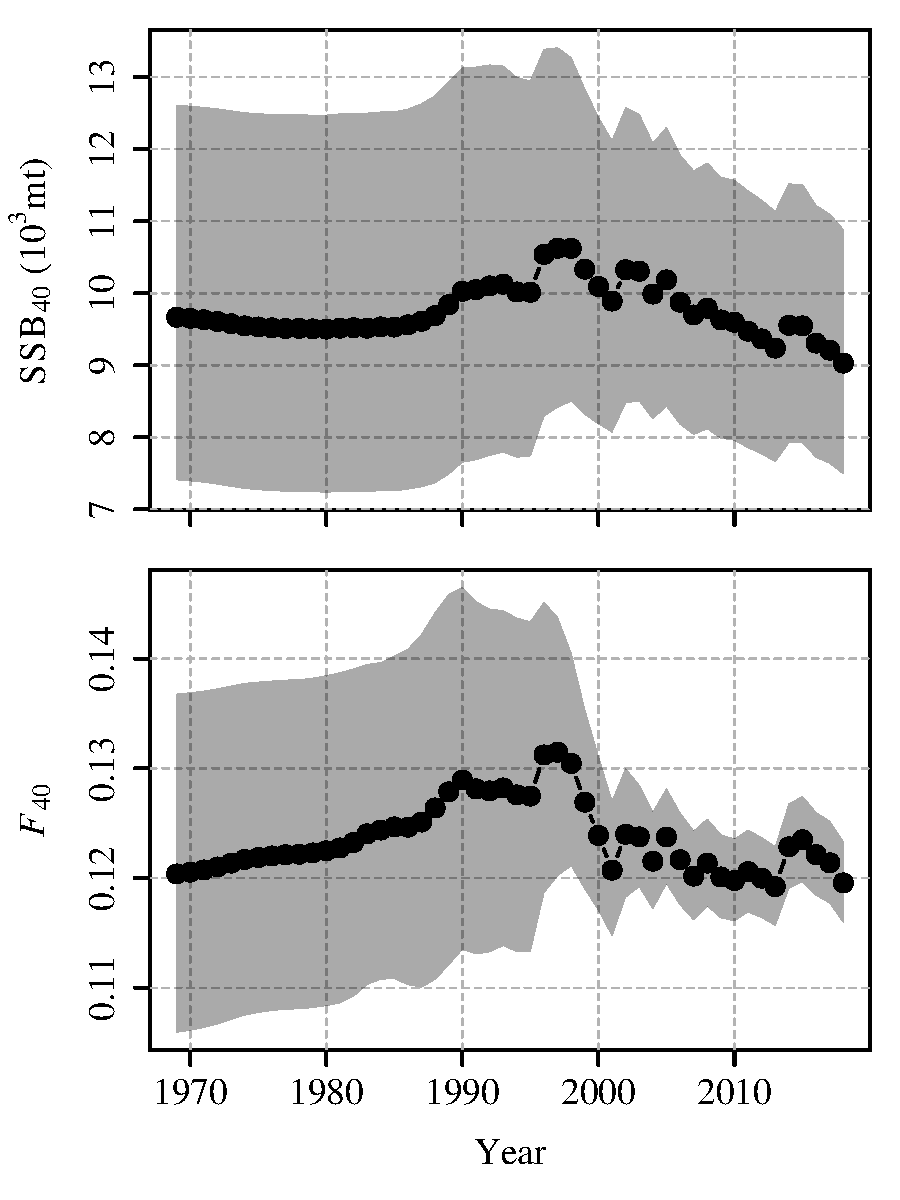
\includegraphics[height = 0.8\textheight]{../results/ssm_temp/petrale_BRPs.pdf}
\end{center}
\end{figure}

\end{document}
